
\documentclass[]{article}
\usepackage{fullpage}
\usepackage{tikz}
\usepackage{tikz,fullpage}
\usetikzlibrary{arrows,%
petri,%
topaths}%
\usepackage{tkz-berge}
\usepackage[position=top]{subfig}
\usepackage{amsmath}
\usepackage{amsfonts}
\usepackage{amssymb}
\usepackage{graphicx}
\usepackage{textcomp}
\usepackage{tabularx}
\usepackage{float}
\usepackage{verbatim}
\usepackage{listings}
\usepackage{xcolor}
\definecolor{DarkGreen}{RGB}{10,132,20}

\lstset{language=R,
basicstyle=\small\ttfamily,
stringstyle=\color{DarkGreen},
morekeywords={TRUE,FALSE},
deletekeywords={data,frame,length,as,character,subset,<-,c,resid,lm},
keywordstyle=\color{gray},
commentstyle=\color{DarkGreen},
}

\title{Template}
\author{Name}
\begin{document}
\maketitle
\section{Preliminaries}
Firstly, before we began and analysis of the data set we created 4 new data frames from the data set to group the patients, T1 and T2 costs by accomodation type using the code below.
\\
\\
It might be useful to take note of the identifiers given to the different data frames as they may appear later on in the document.
\begin{lstlisting}
library(durham)
data(learndis)

domdis <- subset(learndis, ACCOM=="DOM", select = c("PATIENT","COSTS.T1","COSTS.T2"))
hosdis <- subset(learndis, ACCOM=="HOS", select = c("PATIENT","COSTS.T1","COSTS.T2"))
rnhdis <- subset(learndis, ACCOM=="RNH", select = c("PATIENT","COSTS.T1","COSTS.T2"))
sghdis <- subset(learndis, ACCOM=="SGH", select = c("PATIENT","COSTS.T1","COSTS.T2"))
\end{lstlisting}
\section{Numerical Summaries}
\subsection{Summaries}
Below is some R output, displaying the numerical summaries for each of the distributions. In the next section we will use boxplots to visually assess the distributions, with T1 and T2 costs side by side for each of the accomodation types.
\verbatiminput{RStudio/txt/Summaries.txt}
\subsection{Boxplots}
Illustrated by the boxplot below there is an obvious difference between the T1 and T2 costs for domestic accomodation. Both appear to be left skewed, with T2 appearing more left skewed than T1. Both have an outlier but T2 has a very extreme outlier which will need to be considered and may cause problems later on.
\centering
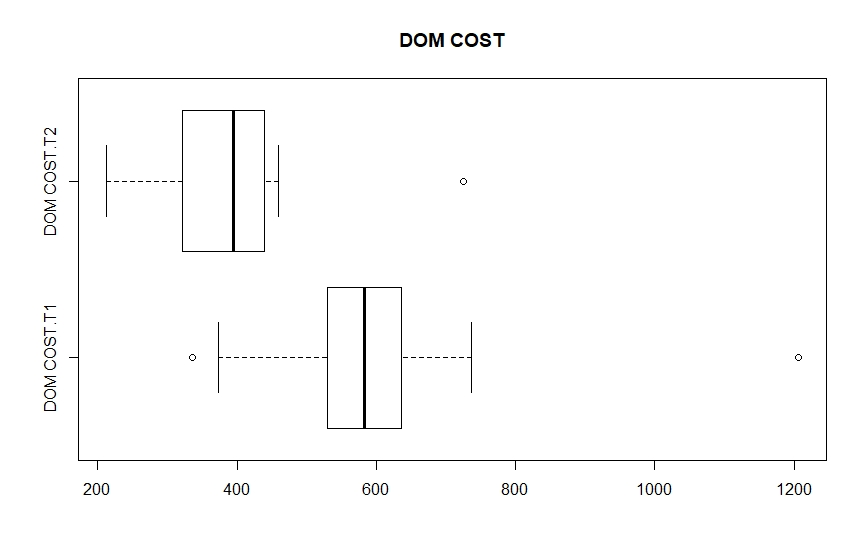
\includegraphics[width=\textwidth]{RStudio/jpeg/Box_DOM.jpeg}
\raggedright
The box plot below shows us that T1 and T2 costs for hostel accomodation are both widely spread. The skew of the either distribution is not obvious from the boxplots, but we can see that in general T1 costs appear to be greater than T2 costs.
\centering
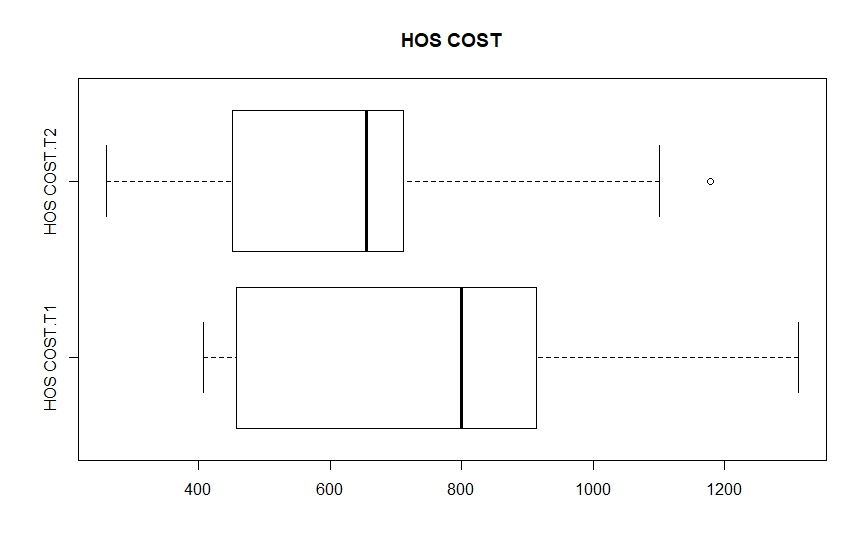
\includegraphics[width=\textwidth]{RStudio/jpeg/Box_HOS.jpeg}
\raggedright

The box plot below shows there is some difference between T1 and T2 costs for residential and nursing homes. T1 costs are alot more widely spread than T2 costs, but T2 costs look very normal at a first glance.
\centering
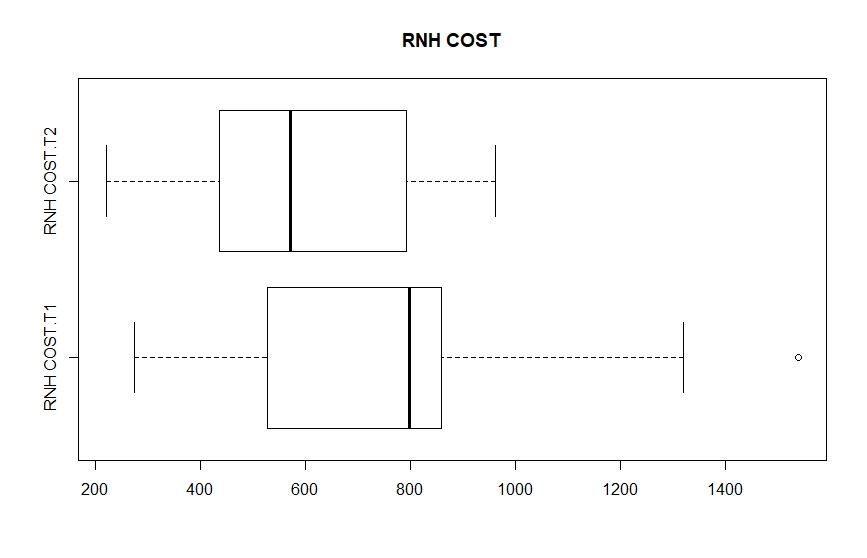
\includegraphics[width=\textwidth]{RStudio/jpeg/Box_RNH.jpeg}
\raggedright

T1 and T2 costs do not seem to differ much for professionally staffed homes. T2 costs are slightly wider spread and T1 costs have 2 outliers, but regardless, they appear to be very similarly distributed.
\centering
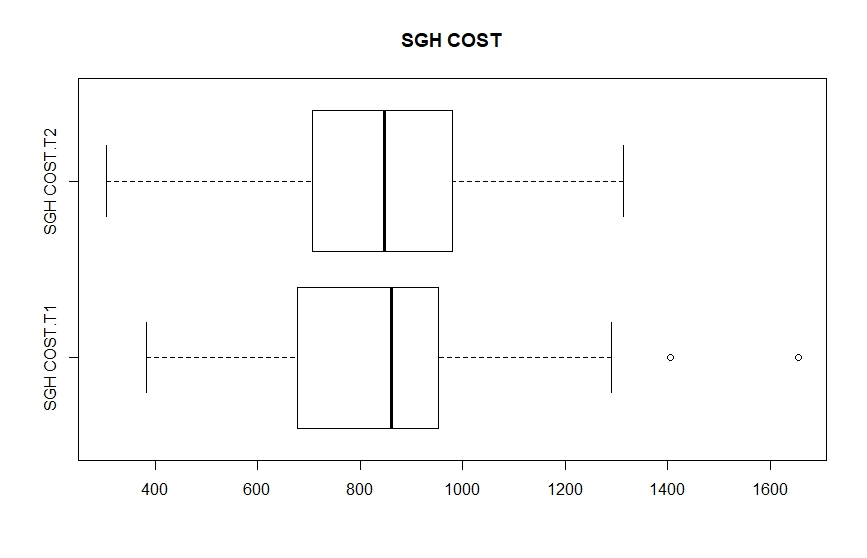
\includegraphics[width=\textwidth]{RStudio/jpeg/Box_SGH.jpeg}
\raggedright

The box plot below shows the distribution for all T1 and T2 costs (regardless of the accomodation type). We can see that in general T1 costs ares higher than T2 costs, and at a first glance both distributions look reasonably normal.
\centering
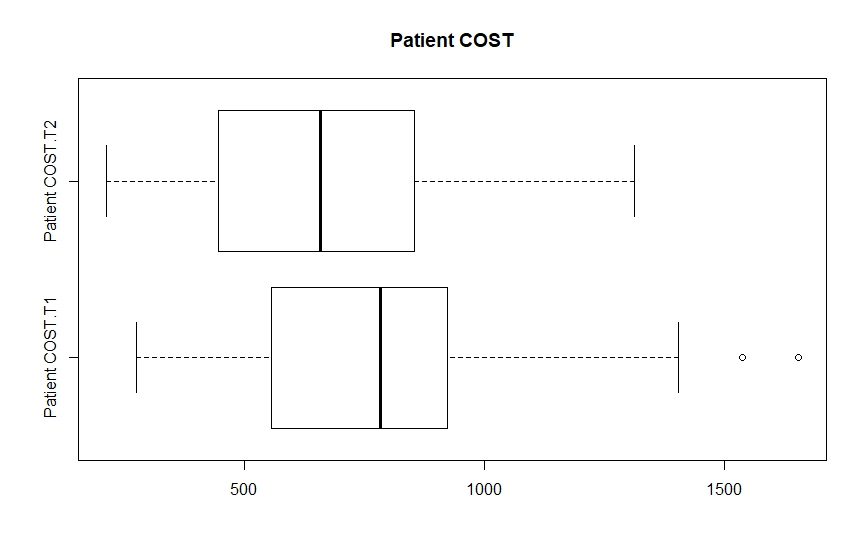
\includegraphics[width=\textwidth]{RStudio/jpeg/Box_COST.jpeg}
\raggedright

\section{Assesment of Normality}
\subsection{Stem and Leaf plots}
The following R output could be used to asses the normality of the different distributions by looking at the shape of the stem and leaf plots. However, we will fully asses the normaility of each distribution in the next section.

\verbatiminput{RStudio/txt/Stem-Leaf.txt}

\subsection{Normal Fit}
The T1 costs for domestic accomodation appear to loosely follow a normal distribution. We have a small n, and excluding the outlier we can see that the bulk of the data follows a linear trend on the normal quantile plot. The histogram also shows some signs of normality, so we could begin to make probabalistic calculations using the normal distribution.

\centering
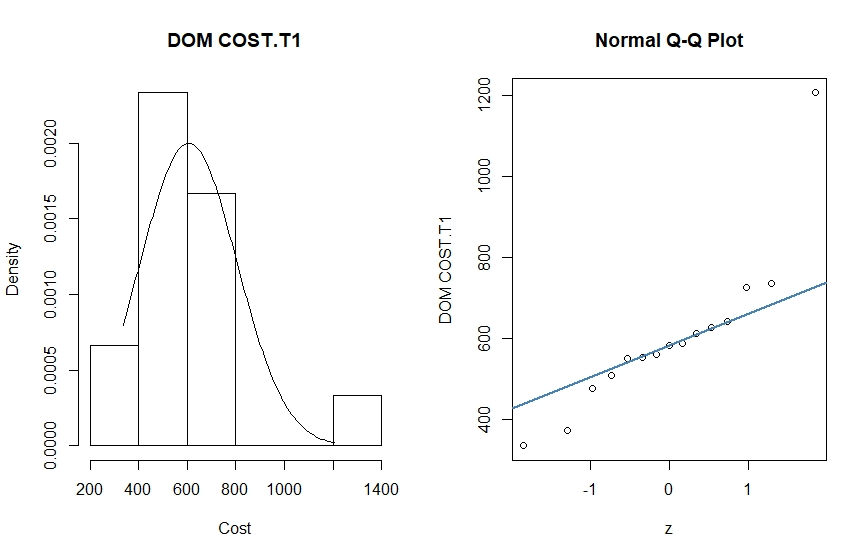
\includegraphics[width=\textwidth]{RStudio/jpeg/Norm_DOM_T1.jpeg}
\raggedright

The T2 costs for domestic accomodation give us a similar situation. We have a small n, and an extreme outlier which can be excluded. On the normal quantile plot all the data follows the same linear trend apart from the outlier, so these costs actually appear even more normal and we could safely say they follow a normal distribution.
\centering
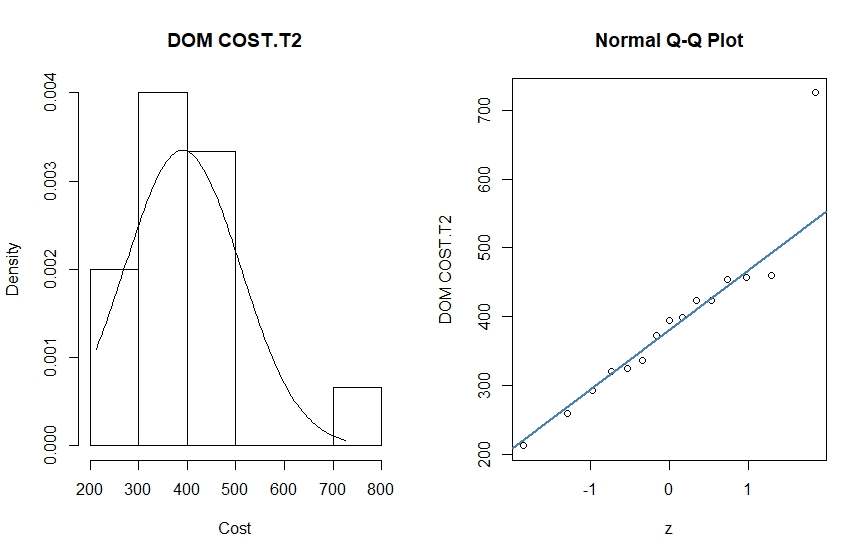
\includegraphics[width=\textwidth]{RStudio/jpeg/Norm_DOM_T2.jpeg}
\raggedright

The T1 costs for hostel accomodation do not appear to follow a normal distribution. The histogram appears bi-modal, and there are systematic devations from the straight line on the normal quantile plot. Perhaps there is some other variable that has not been considered or the sampling was bias.
\centering
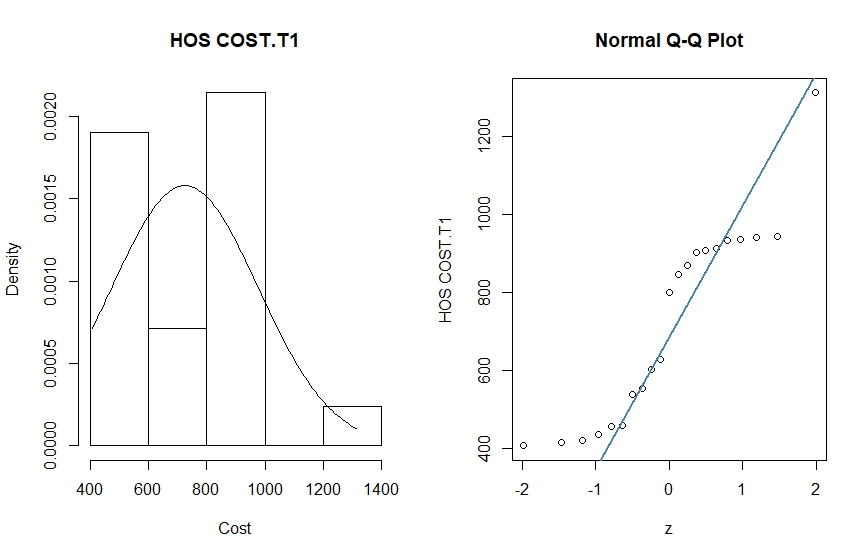
\includegraphics[width=\textwidth]{RStudio/jpeg/Norm_HOS_T1.jpeg}
\raggedright

For the T2 costs for hostel accomodation we see something different. The histogram appears to be reasonably normal, however the normal quantile plot shows clustering around certain values. Because the histogram does not show the 'full picture' we can say this distribution is again not normal, because the normal quantile plots suggests it isn't.
\centering
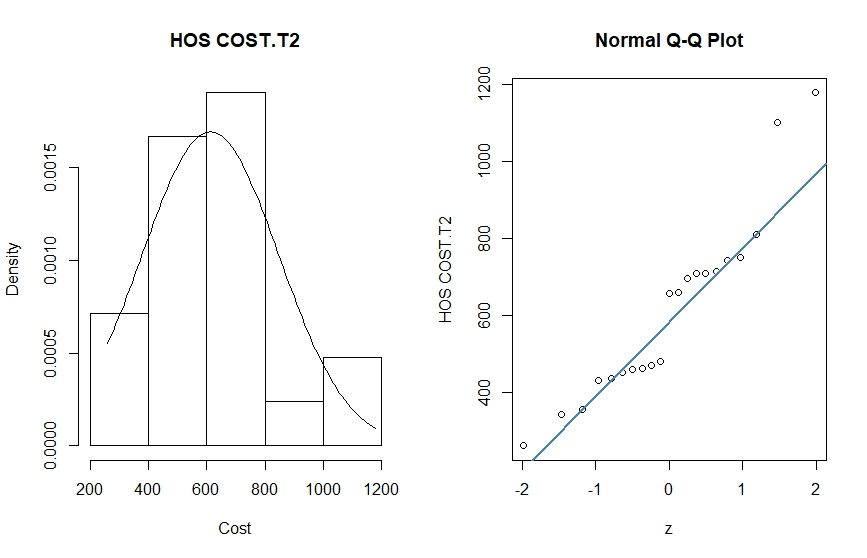
\includegraphics[width=\textwidth]{RStudio/jpeg/Norm_HOS_T2.jpeg}
\raggedright

The T1 costs for residential and nursing homes appear to follow a normal distribution. The histogram is slightly right skewed but appears fairly normal, and the points in the normal quantile plot roughly follow a linear relationship without too much clustering or deviation from the straught line.
\centering
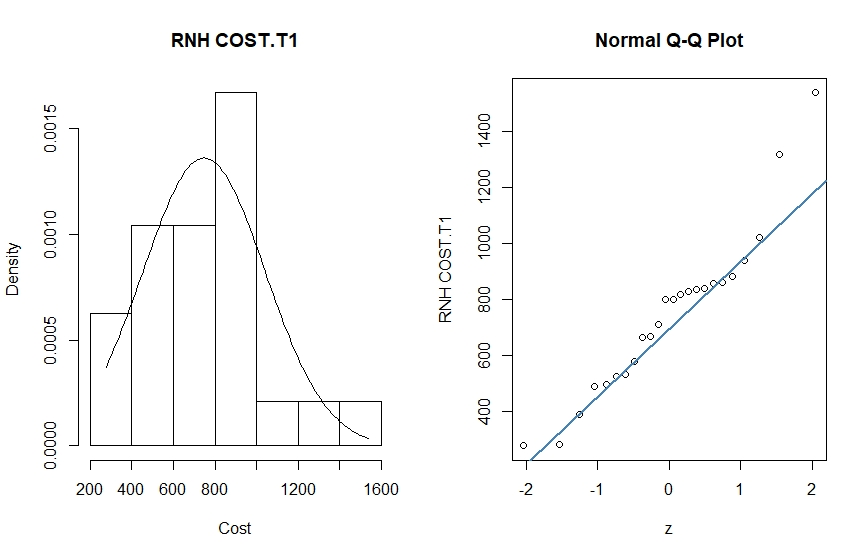
\includegraphics[width=\textwidth]{RStudio/jpeg/Norm_RNH_T1.jpeg}
\raggedright

For the T2 costs for residential and nursing homes we get a strange histogram. We appear to have quite large tails but the distribution still seems to be fairly symmetric. The points on the normal quantile plot roughly follow a linear relationship with not not too much deviation from the line except at the tails. We could use a normal distribution but we would have to be careful, perhaps a t-distribution would be more suitable because of our large tails.
\centering
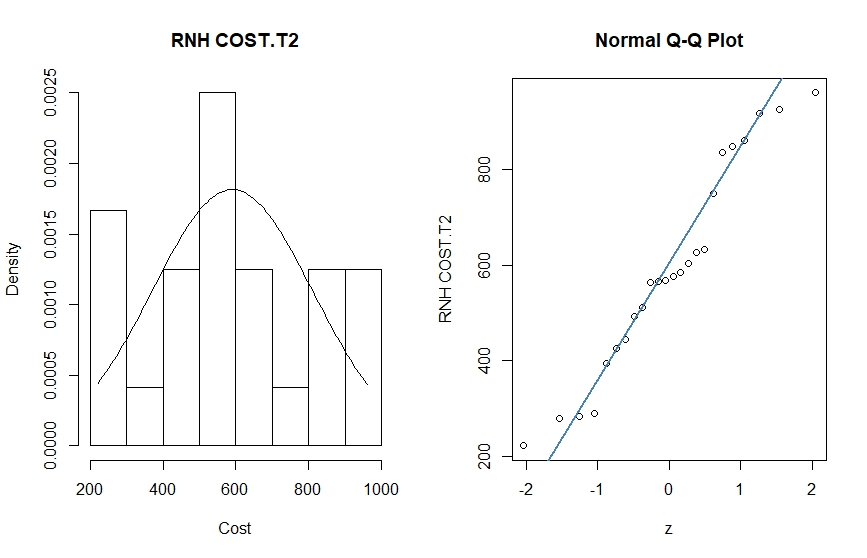
\includegraphics[width=\textwidth]{RStudio/jpeg/Norm_RNH_T2.jpeg}
\raggedright

The T1 costs for professionally staffed homes appear to follow a normal distribution quite closely. The histogram looks very normal (only slightly right skewed), and the points on the normal quantile plot closely follow a linear relationship apart from the few outliers. This could because we have a relatively large n for professionally staffed homes.
\centering
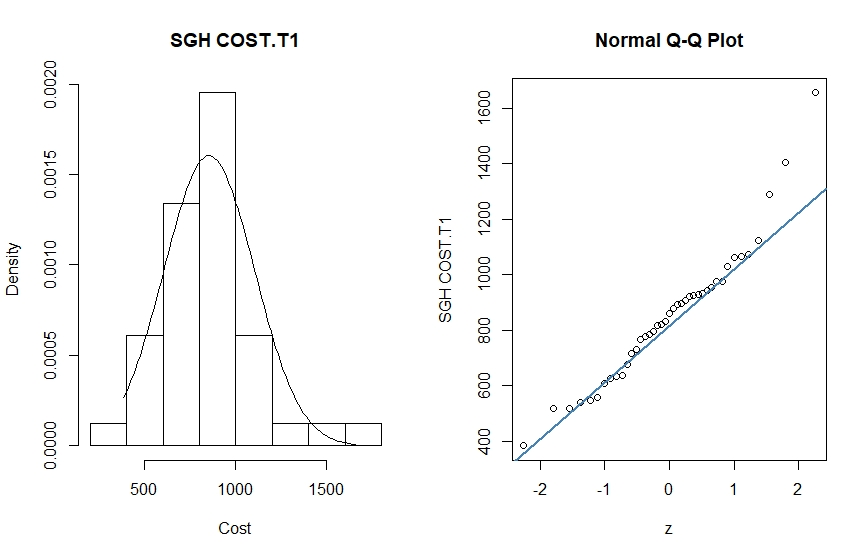
\includegraphics[width=\textwidth]{RStudio/jpeg/Norm_SGH_T1.jpeg}
\raggedright

We get a similar situation for the T2 costs for professionally staffed homes. The histogram again looks quite normal, however it is left skewed in this case. The points on the normal quantile plot again closely follow a linear relationship apart from some of the smaller values.
\centering
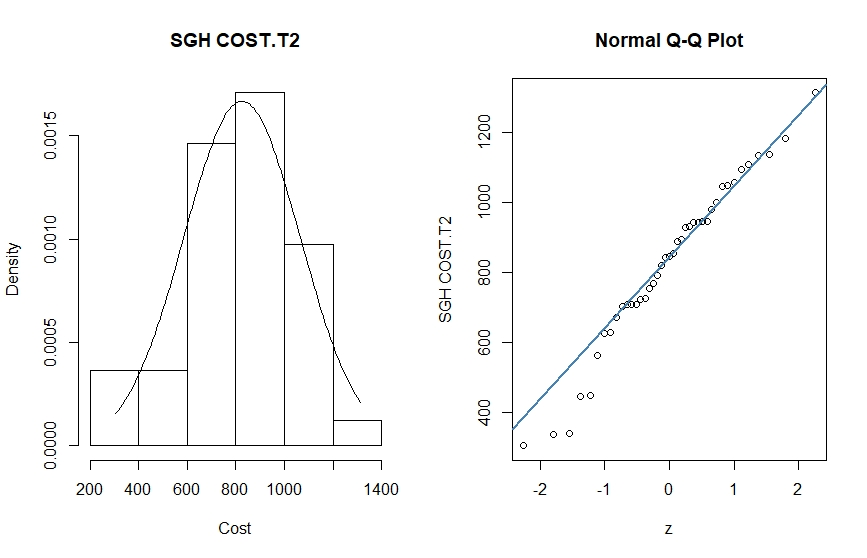
\includegraphics[width=\textwidth]{RStudio/jpeg/Norm_SGH_T2.jpeg}
\raggedright

The plots below are for the T1 costs of all patients regardless of the accomodation type. We can see some signs of normality; on the normal quantile plot a large bulk of the data follows some linear trend, but we have some systematic deviations at the tails. Overall the histogram shows some normality but the distribution appears to be right skewed. We would need to be careful if we use a normal distribution to model this data, perhaps some transformation could help us.
\centering
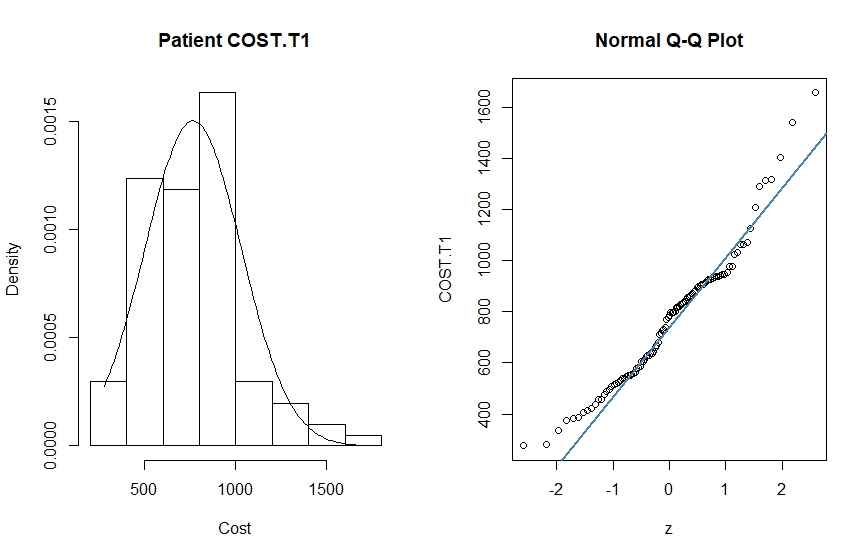
\includegraphics[width=\textwidth]{RStudio/jpeg/Norm_T1.jpeg}
\raggedright

Below are the plots for the T2 costs of all the patients and accomodation types. Our histogram appears bimodal so a normal model would be unwise. However, our normal quantile plot seems to suggest reasonable normality for the data. Most of the points follow the same linear trend with the tails being exceptions, there seems to be less systematic deviation in the normal quantile plot, but it would still be risky to use a normal distribution to model this data. The bimodality of the histogram suggests there is anither underlying variable that has not been considered, a transformation could also be used.
\centering
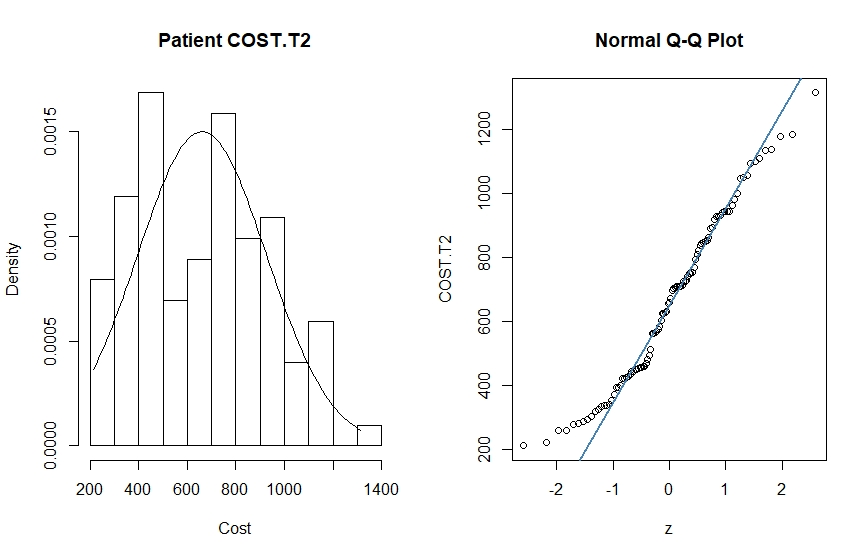
\includegraphics[width=\textwidth]{RStudio/jpeg/Norm_T2.jpeg}
\raggedright


\section{Associations}
\subsection{Linear Models}
Below is the R script that creates linear models for predicting costs at T2 from costs at T1 for every accomodation type and for the overall data set.
\begin{lstlisting}
lmdom <- lm(domdis$COSTS.T2~domdis$COSTS.T1)
lmhos <- lm(hosdis$COSTS.T2~hosdis$COSTS.T1)
lmrnh <- lm(rnhdis$COSTS.T2~rnhdis$COSTS.T1)
lmsgh <- lm(sghdis$COSTS.T2~sghdis$COSTS.T1)
lmdis <- lm(learndis$COSTS.T2~learndis$COSTS.T1)
\end{lstlisting}
Below is the R output for the summaries of each of the linear models

\verbatiminput{RStudio/txt/Linear-Model-Summaries.txt}

The below graph plots T2 costs against T1 costs for domestic accomodation with a regression line. There is a weak positive correlation but it is clear there is little association between the 2 varibales from the graph and notably the R value is only 0.03323
\centering
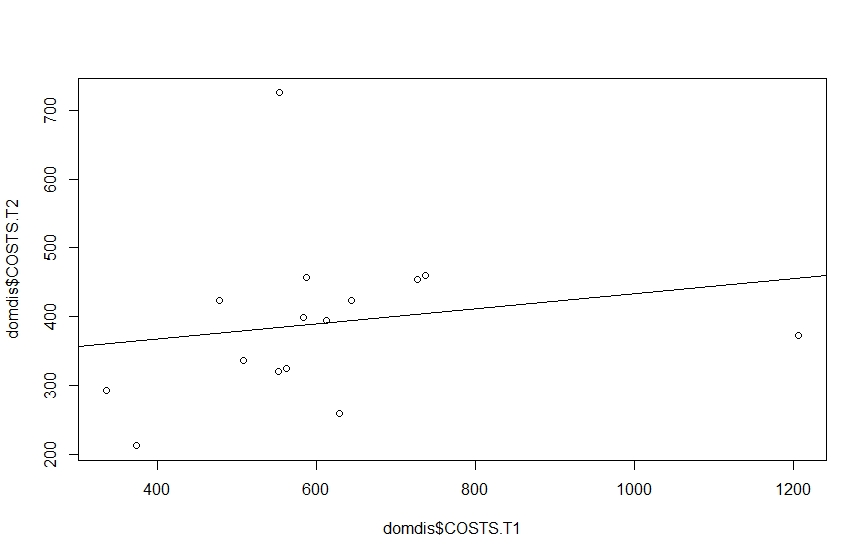
\includegraphics[width=\textwidth]{RStudio/jpeg/Reg_DOM.jpeg}
\raggedright

The below graph plots T2 costs against T1 costs for hostel accomodation with a regression line. There appears to be an incredibly weak negative correlation, with 2 seperate clusters of points, so again there is little association between the variables.
\centering
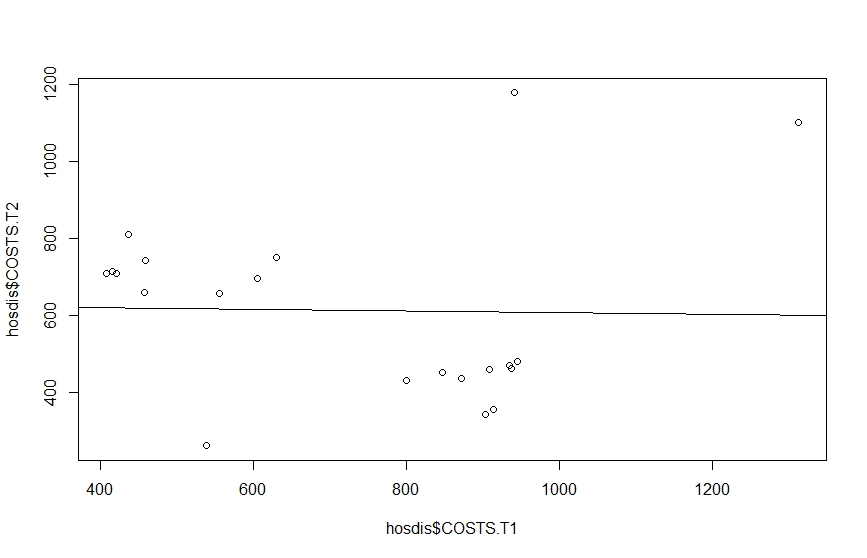
\includegraphics[width=\textwidth]{RStudio/jpeg/Reg_HOS.jpeg}
\raggedright

The next graph plots T2 costs against T1 costs for residential and nursing homes. Theres appears to be some positive correlation, but again it is weak. Infact it is the strongest linear model with an R value of 0.1275.
\centering
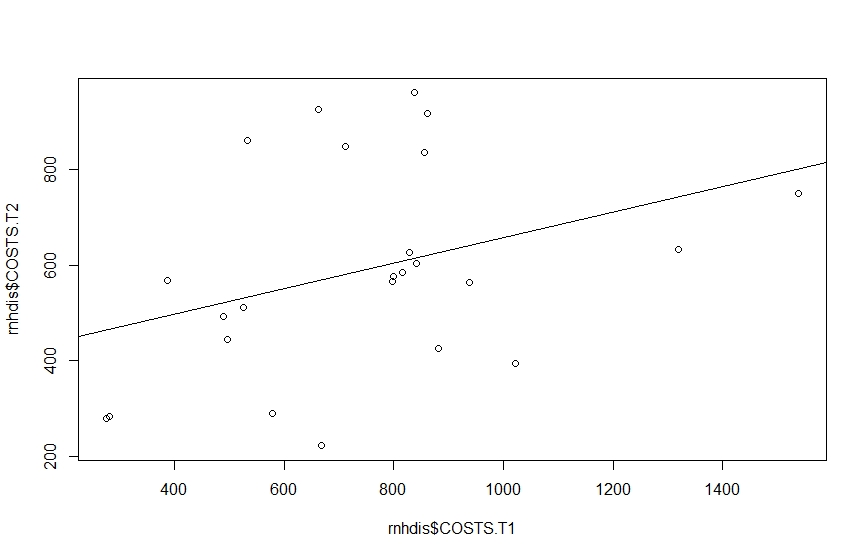
\includegraphics[width=\textwidth]{RStudio/jpeg/Reg_RNH.jpeg}
\raggedright

The next graph plots T2 costs against T1 costs for professionally staffed homes. There appears to be np correlation at all and an R value of 5.649e-05, would indeed suggest there is no association between the 2 variables.
\centering
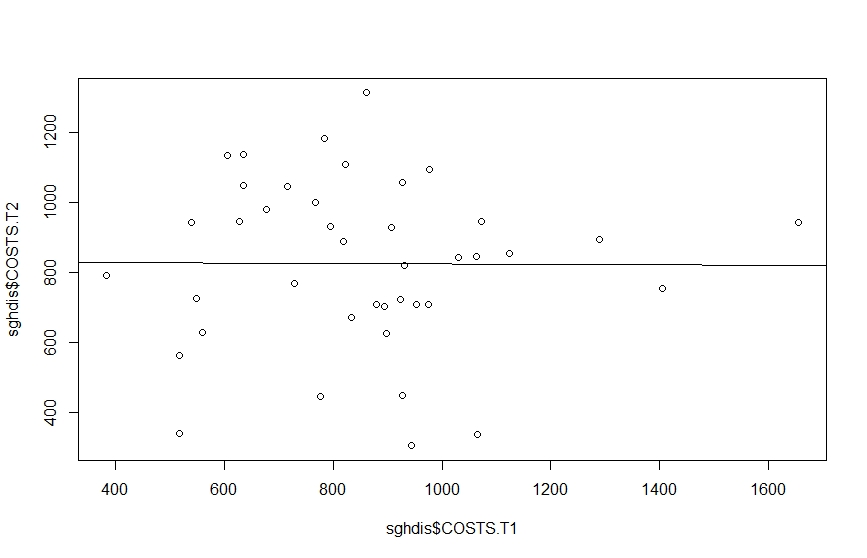
\includegraphics[width=\textwidth]{RStudio/jpeg/Reg_SGH.jpeg}
\raggedright

The final graph shows all the T2 costs against all the T1 costs for all the accomodation types. There appears to be a positive correlation but it is weak with an R value of 0.06935, so there is a weak association between the variables.
\centering
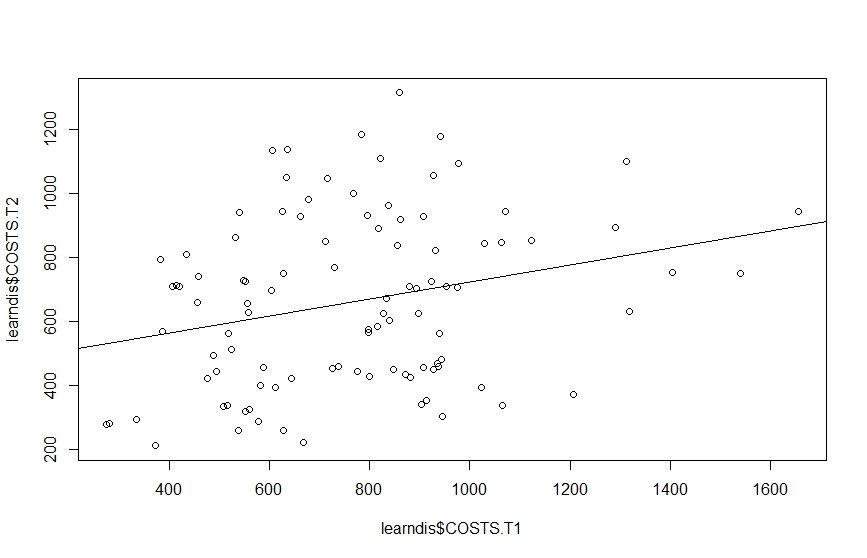
\includegraphics[width=\textwidth]{RStudio/jpeg/Reg_COST.jpeg}
\raggedright


\section{Stability of Associations}
\subsection{Residuals}
The below R script stored the residuals of the linear models in some variables.
\begin{lstlisting}
residdom <- resid(lmdom)
residhos <- resid(lmhos)
residrnh <- resid(lmrnh)
residsgh <- resid(lmsgh)
residdis <- resid(lmdis)
\end{lstlisting}
\begin{flushleft}
The following commentary will be breif because we already assessed the normality of the distributions previously, and assesing the normality of the residuals will give us the same results as the T2 costs. A residual plot is also provided as an alternate way of visually assesing the normality of the residuals for each of the T2 costs.
\end{flushleft}

The residulas below for domestic accomodation are normal. So any probabalistic statements made are valid.

\centering
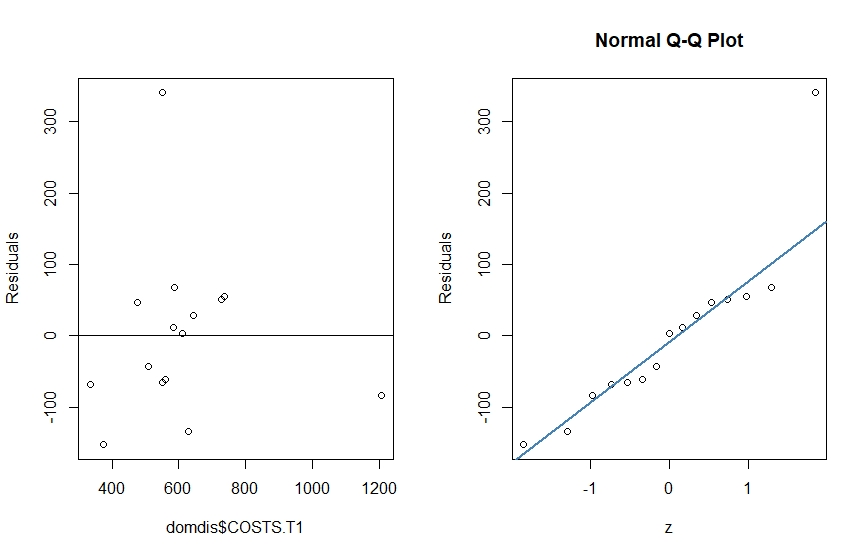
\includegraphics[width=\textwidth]{RStudio/jpeg/Res_DOM.jpeg}
\raggedright

The residuals below for hostel accomodation are not normal. So any probabalistic statements made are not valid.
\centering
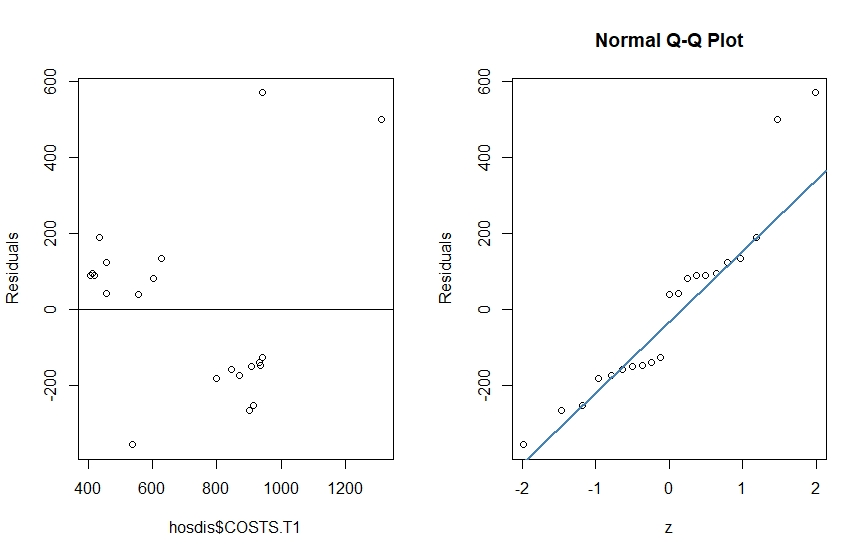
\includegraphics[width=\textwidth]{RStudio/jpeg/Res_HOS.jpeg}
\raggedright

The residuals below for residential and nursing homes are not normal.
\centering
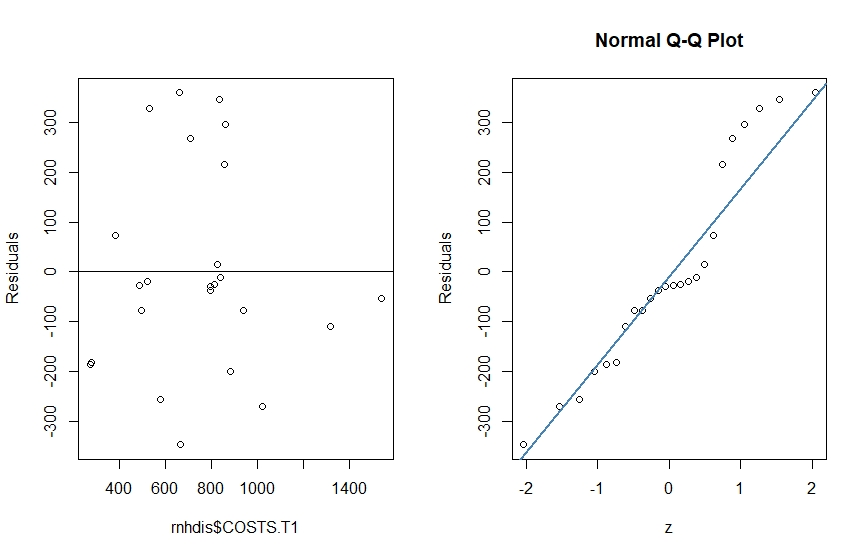
\includegraphics[width=\textwidth]{RStudio/jpeg/Res_RNH.jpeg}
\raggedright

The residuals below for professionally staffed homes are normal.
\centering
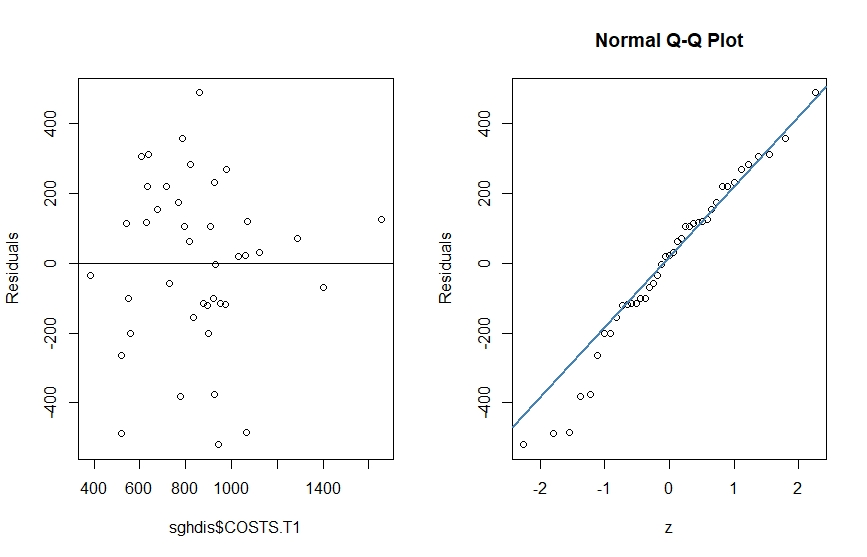
\includegraphics[width=\textwidth]{RStudio/jpeg/Res_SGH.jpeg}
\raggedright

The residuals below are for all T2 costs for all accomodation types. For the majority of the data they are normal, but the tails deviate slightly. We must be careful but we could say any probabalistic statements are valid.
\centering
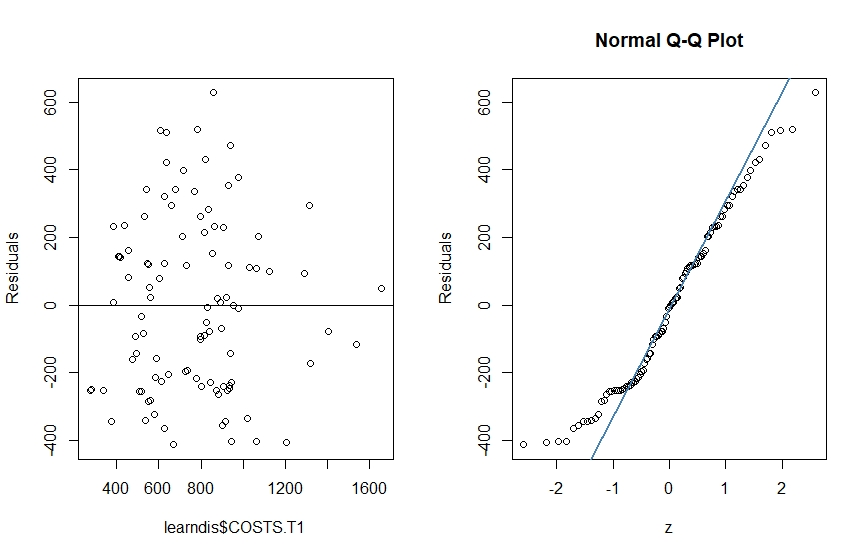
\includegraphics[width=\textwidth]{RStudio/jpeg/Res_COST.jpeg}
\raggedright

\section{Conclusions}

\end{document}



